\chapter{設計と実装}
\label{chap:implementation}
\section{実験概要}
\section{1人麻雀プレイヤーの設計と実装}
提案手法で提示した、期待和了平均順目の評価によるモンテカルロ木探索を評価するために、1人麻雀プレイヤーを実装した。
1人麻雀プレイヤーとは、相手プレイヤーを考えない多人数性を排除した麻雀のことである。ルールについては次の節で詳しく説明している。
本研究で実装した1人麻雀プレイヤーのフローチャート図を図\ref{flow1}に示す。
まず、1人麻雀プレイヤーにおいて開局から、終局まで行う対局のループを定義する。
開局時には、山と配牌を設置する。その後山から一つ牌をツモり、一つ捨てる動作を繰り返す。終了条件を満たした時点で終局となり、その局の成績を集計する。このループを1人麻雀プレイヤーにおける1対局と定義する。この対局のループを十分な回数行い、和了率を測定する。

% 期待和了平均順目をn順先の変化まで評価することによって性能が変わる可能性があるので、1順、2順、3順までの変化を考慮するものをそれぞれ分けて実験した。
% それぞれに対して100局のテストデータと10,000局のテストデータを与え、あがることができた局数を計測した。テストデータとは、全ての牌をランダムに並べたものを100セット用意したデータである。このデータから 13 牌を初期牌として 与え, その後牌を引いて切る動作を 27 回行い, その中であ がれたかどうかを確認した。100 局のテストデータで人間 のプレイヤとの比較を行い, 10,000 局のテストデータで各 手法の性能の評価を行った。

\begin{figure}[h]
 \centering
 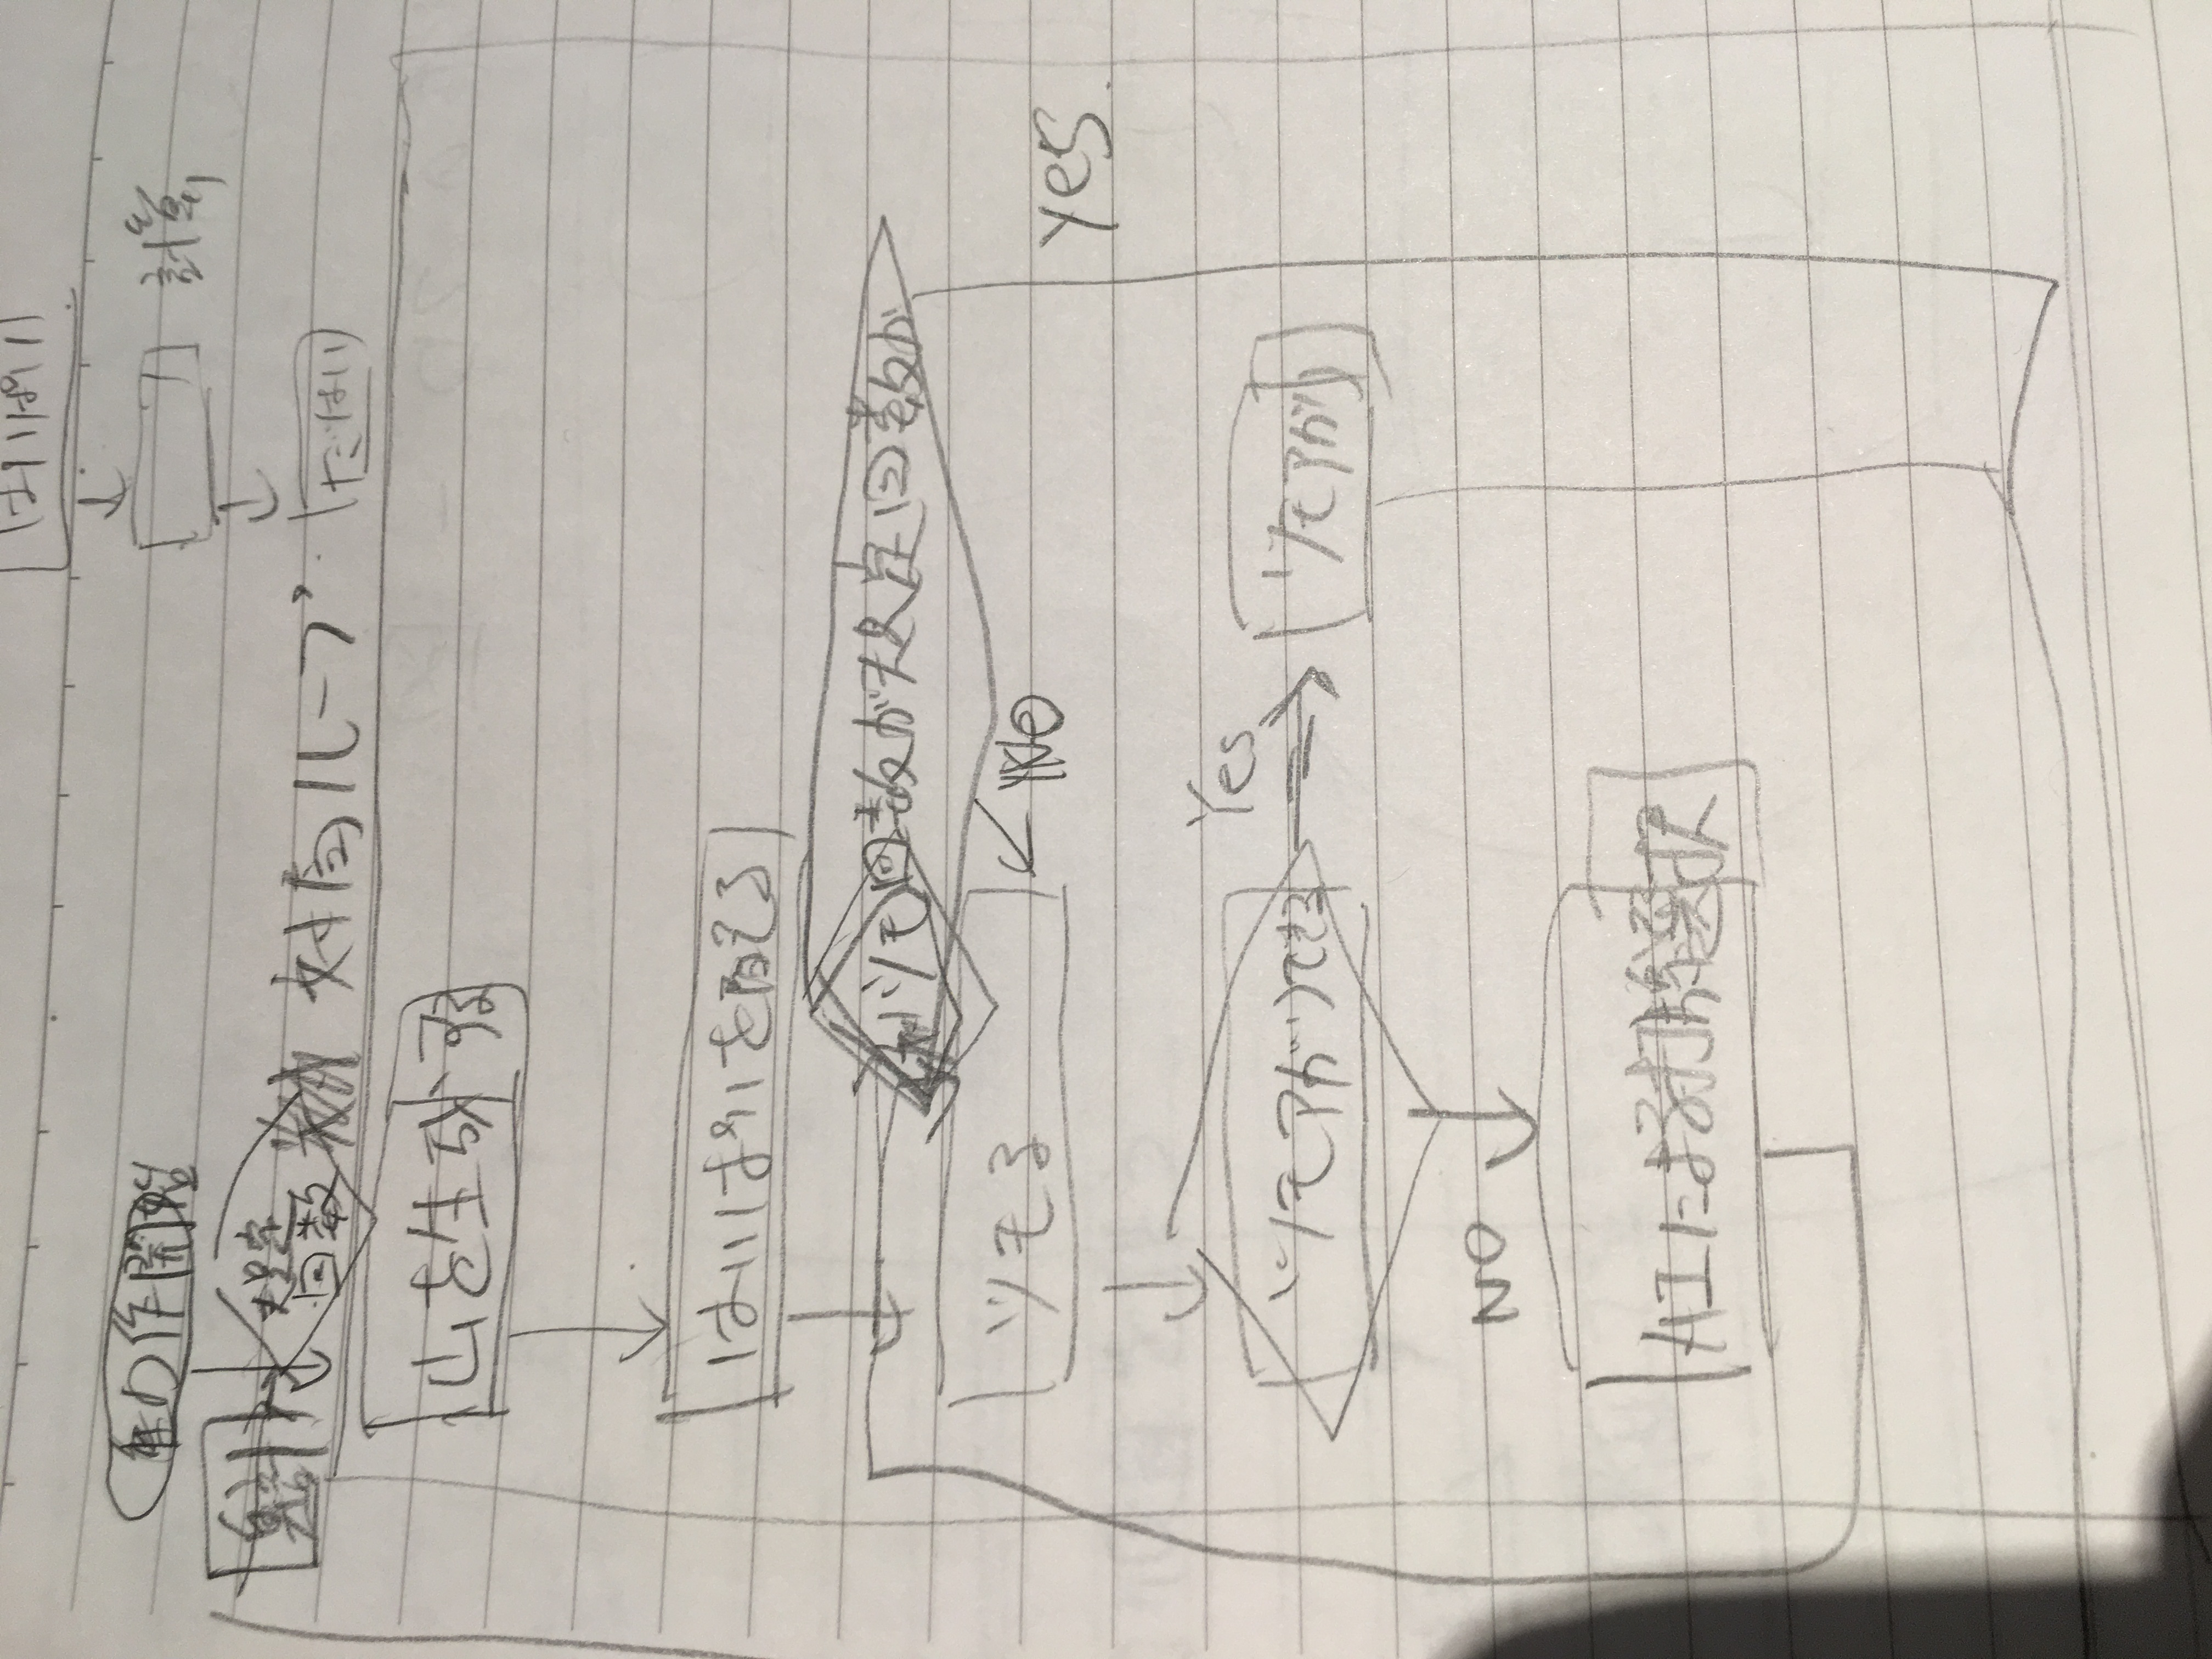
\includegraphics[keepaspectratio, scale=0.1,bb=0 0 3024 4032]
      {img/flow.jpg}
 \caption{1人麻雀のフローチャート}
 \label{flow1}
\end{figure}

\section{1人麻雀のルール}
多人数ゲームでは状況によってプレイヤの行動の目的が違うといった難しさがある。この難しさを解消するために、相手を考慮しない1人麻雀プレイヤを考える。
この1人麻雀プレイヤのルールは、相手プレイヤを考えないため、相手プレイヤーに点数を支払う事による放銃や被ツモ失点などを考えない。また、相手プレイヤーによる捨て牌が存在しないので、鳴きや栄和を考えない。リーチについても、和了率の観点では不要なため、考えない。門前でツモを繰り返し行うだけのシンプルなシステムである。先行研究\cite{bakuuti}評価を合わせるため、ツモの回数は 27 回とした。

\begin{table}[htbp]
  \caption{本研究の1人麻雀プレイヤのルール}
  \label{tb:bakuuti_score}
  \begin{center}
  \begin{tabular}{c|c|c}
    \hline
    アクション  & 4人麻雀 & 1人麻雀 \\\hline\hline
    和了  & ツモ和了、ロン和了どちらも可 & ツモ和了のみ\\\hline
    点数 & 失点や和了の点数を考慮する & 点数は考えない\\\hline
    リーチ & 可能 & なし\\\hline
    鳴き & チー、ポン、カンが可能 & なし\\\hline
    終局 & 誰かが和了するか、ツモ山70枚がなくなるまで(136-14-13*4) & 和了するか、27回ツモるか\\\hline
  \end{tabular}\end{center}
\end{table}

また1人麻雀の成績の評価においてはその点数の推移よりも、和了率自体が重要だと考えられている。したがって、点数という複雑なパラメータを省いた和了率に注目したルールとなっている。その理由としては、以下のような理由が述べられる。

まず、4 人麻雀では平均順位の低いプレイヤほ ど、平均和了点低く、和了率が高いことが統計で明ら かになっている\cite{kagaku}したがって強いプレイヤは点数よりも和了率を重視して打っていることがわかる。

上手いプレイヤの平均和了点が低くなる理由として手役を無理に狙った打ち方をしないためで
ある。また麻雀の点数の特性上、満貫までの点数は指数関数的にその得点が増えていくが、満貫以上の場合は線形に近くなる。したがって、難易度に対して望める点数が割に合わない高い和了を狙うより、比較的低い点数で゙多く和了することが効率が良い。
また、失点の観点からも、4人麻雀では自分が放銃をしない場合も他プレイヤーの和了によって被ツモ失点を被ることがある。これに対しても、和了すれば他プレイヤーが和了することができないため、相手のチャンスをつぶすといった意味でも和了率の高さは大事である。

\subsection{終了条件}
・ツモが規定回数かどうか
・そもそもなんでツモ回数を27としてるのか?



\subsection{全体のループ回数}

\subsection{山のデータセット}
同じように用意したもの

\subsection{AIによる打牌選択}
・どのような手法を選択したか
爆打モンテカルロ法
UCB1モンテカルロ法
LinUCBを用いた方法
・どのように実装したか どのような制限を加えたか
(プレイアウトの回数、CPUや実装コード)
計算量の問題

\subsection{シャンテン数の計算方法}
バックトラック法、ハッシュ法




% \subsection{期待平均和了順目の探索の深さの評価}
% \subsection{モンテカルロ法の探索領域}


\section{4人麻雀における実対戦用システム} %麻雀サーバーとの対戦
本研究の提案手法のアルゴリズムが4人麻雀でも有用かどうかを調べるために、4人麻雀で実際に対戦するための自動打ちシステムを構築した。このシステムを動かす場所として、オンライン麻雀サイト「天鳳」を選んだ。

・環境
・VM上
% 本研究では1人麻雀における和了率の向上を目指すため、和了率の数理的評価とモンテカルロ法を適用する部分を限定する手法をとった。佐藤らは、1人麻雀における和了率を有効牌を数え上げて大きくなるようにすることで、和了率の最大化を図り、これを4人麻雀で打たせレートを取った。同じように本研究手法でも4人麻雀で打たせた結果を比較した。

\begin{figure}[h]
 \centering
 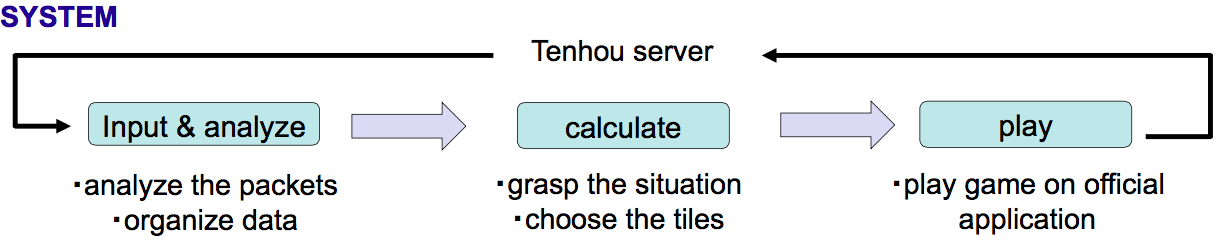
\includegraphics[keepaspectratio, scale=0.3,bb=0 0 1226 243]
      {img/imp1.png}
 \caption{天鳳上で自動打ちするためのシステムの設計図}
\end{figure}

\subsection{オンライン麻雀サイト天鳳}
天鳳は、現在インターネット上で麻雀を打つことができるサイトの中で最も利用者が多いサイトであり、登録者は390万人を超える大型のサイトである。また、アクティブユーザー(180日以内の対戦履歴があるプレーヤ数)は27万人を超え、現在最も活気のあるインターネット上の麻雀フィールドである。天鳳では麻雀研究に対する支援が充実しているという面も大きい。
最高ランク者のみが打つことのできる鳳凰卓というクラスの試合データ(以下牌譜)を全て公開しており、より良質な強者の牌譜を取得することができる。これらの牌譜は一日に約500試合ほど手に入り、量ともに十分利用できる。これについては、筆者も強者の統計的な手順について研究する際によく利用させていただいた。また、天鳳ではAIで麻雀を打つことを一定の条件下で許可している点も大きい。鳳凰卓については人間同士の生粋の強者のフィールドというコンセプトがあるため許可されていないが、その下の特上卓以下では条件を揃えることで対戦することが可能である。
一番下の一般卓については、最も低ランクなため対戦人数も多いため、AIによる影響が少ないと考えられている。そのためある程度対戦が可能なAIであれば、他プレイヤーの迷惑にならないような範囲での利用が許可されている。また、一般卓と鳳凰卓の間の上級卓・特上卓では、AIを用いて他のプレイヤーの不正検出に協力するという条件を元にAIの稼働を許可されている。AIを稼働させることによる他プレイヤーのメリットを提供することで、反対するものが少なくなるからである。本研究のシステムは、一般卓で稼働させた。


\begin{figure}[h]
 \centering
 
\includegraphics[keepaspectratio, scale=0.5,bb=0 0 620 439]
      {img/zu.jpg}
 \caption{ランク別リスト・AI稼働条件}
 \label{zu}
\end{figure}

\subsection{プレイさせた天鳳のルール}
・ルールフロー図
・・天鳳上の制約(ルール)
・天鳳上の制約(マシン上の問題 持ち時間)

\section{全体フローの詳細説明}

\section{パケット入力(input)}
・Kmo2さんのやつを利用
・どのようにパケットを読んでるか?
(長く解説する必要はないかもしれない)

\section{計算(後ほど詳しく説明)}
・天鳳からの情報をどういうふうな構造体で保存しているかどうかとか。

\begin{figure}[h]
 \centering
 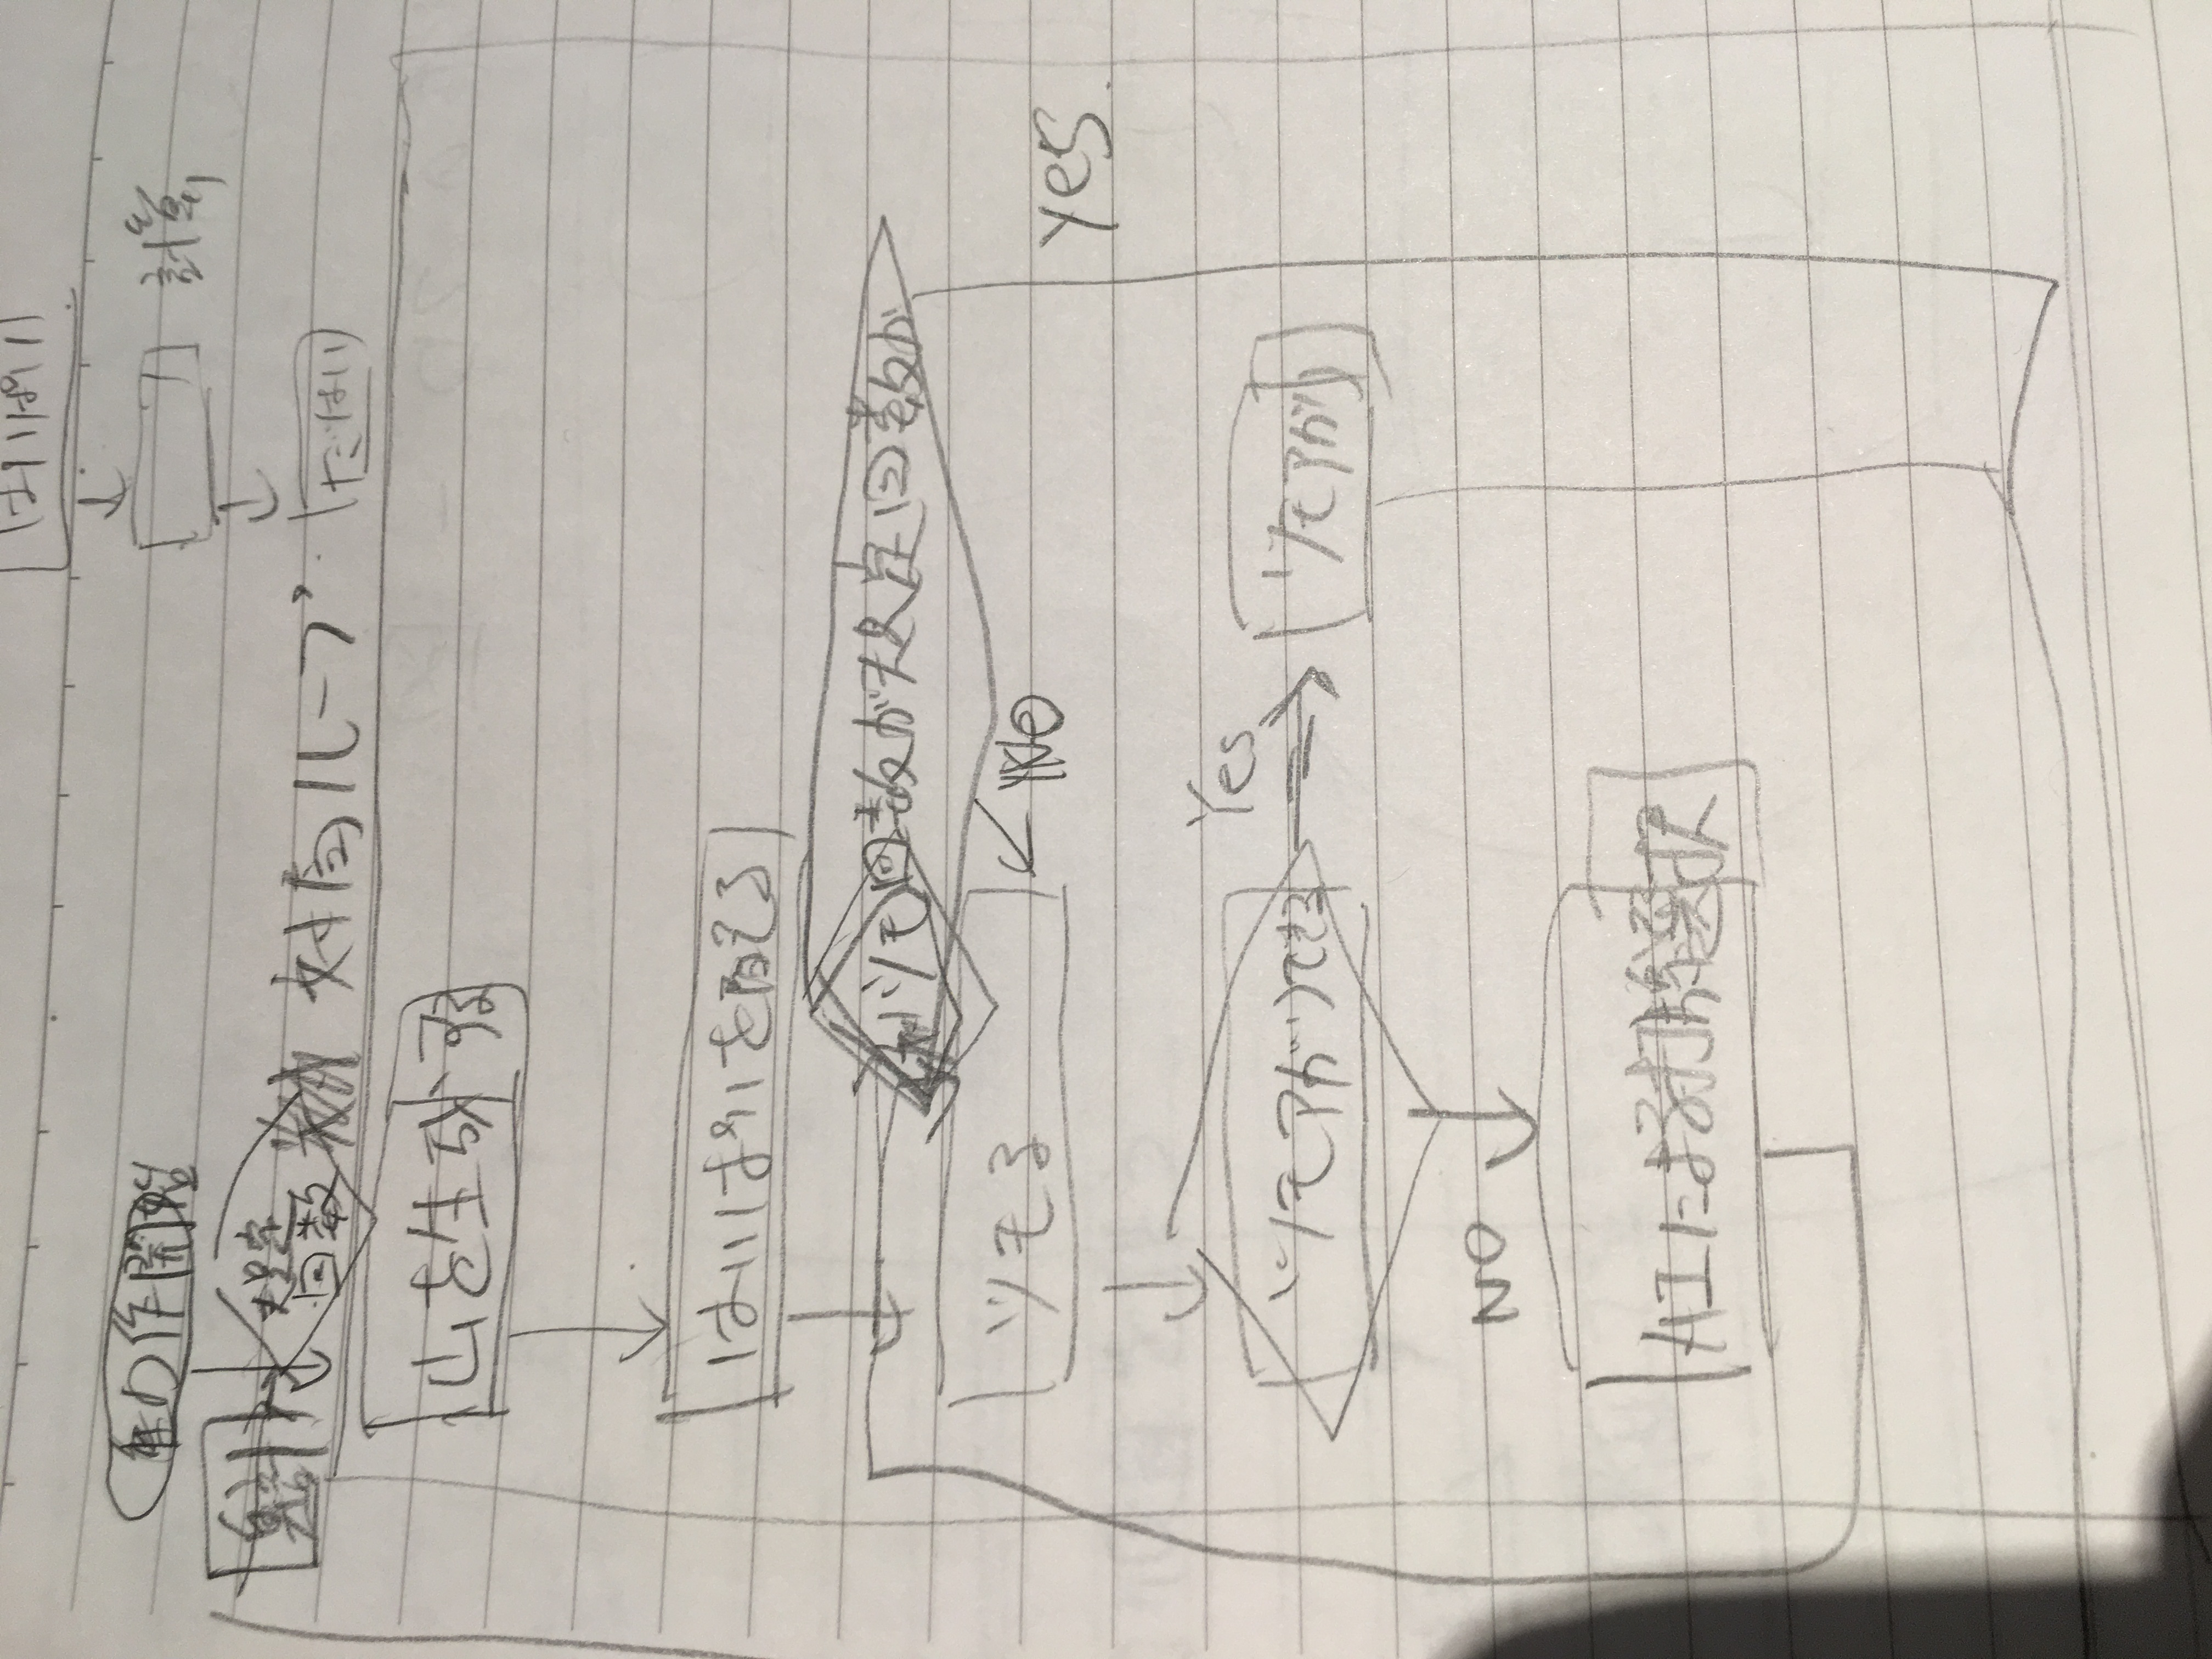
\includegraphics[keepaspectratio, scale=0.1,bb=0 0 3024 4032]
      {img/flow.jpg}
 \caption{4人麻雀自動打ちシステムのフローチャート}
\end{figure}

\subsection{シャンテン数の計算方法}
バックトラック法、ハッシュ法

\section{アウトプット}
・打牌を選択して、天鳳サーバーにそれを送る
・公式クライアントを使うので、マウスハンドラを使う
・配列でどの牌を切るかを選択した上で、左から何番目かを考えてクリックさせる
・リー牌に対してのアクション


